\chapter{Keretrendszer}

\section{Rendszerarchitektúra áttekintése}

Az áramérzékelők (áramváltó bilincsek) mérik az elektromos áramot és az 
adatokat egy ESP8266 gyűjti, ezek pedig a központi vezérlőhöz táplálják, 
amely vezérlőparancsokat küld visszafelé az elektromos járművek töltőinek 
a megengedett áram beállításához.

Az ESP8266-alapú érzékelőcsomópontok mindegyik elektromos töltőnél el vannak helyezve, 
hogy valós időben mérjék a töltőáramot.
Ezek pedig Wi-Fi-n keresztül küldik el az adatokat egy Python Flask alkalmazást futtató 
vezérlőhöz, amely összesíti a méréseket és kiadja a vezérlőparancsokat.

Maguk az töltők Modbus kommunikációval rendelkeznek, ezért a Modbus protokollon keresztül fogadják a 
távolról érkező utasításokat (esetünkben a megengedett áram beállítását).
Mindegyik töltő saját címmel rendelkezik a soros hálózaton.

Az ESP8266 csomópontok csak az adatok két oldalú továbbadásáért felelősek, aktuális adatokat küldenek a 
szervernek, míg a Flask szerver döntéshozatalt hajt végre és parancsokat ad ki a töltőknek.
Az érzékelés és a vezérlés szétválasztása leegyszerűsíti a végpont tervezését 
és a feldolgozást a szerver oldalon központosítja, ami növeli a robosztusságot.

A Flask szerver egy Prometheus idősoros adatbázissal dolgozik 
(ami külön konténer alapú szolgáltatásként fut), ez naplózza az összes mérést 
a megfigyeléshez és elemzéshez. Az összes kiszolgálóoldali összetevő (a Flask alkalmazás, a Modbus 
interfész és a Prometheus) a Docker használatával van konténerben tárolva a 
felhőalapú környezetben történő egyszerű telepítés érdekében. Az architektúra a 
következőket tartalmazza:

\begin{itemize}
    \item ESP8266 érzékelő csomópontok: 
    Wi-Fi csatlakozású mikrokontrollerek minden végponton (legyen az töltő, megszakító, stb\dots), 
    amelyek a csatlakoztatott érzékelőkön keresztül mérik a váltakozó áramot.
    \item Wi-Fi hálózat: Ami biztosítja, 
    hogy a végpontok tudjanak kommunikálni a központi szerverrel. 
    Mindegyik csomópont csatlakozik a helyi Wi-Fi-hez 
    és HTTPS-kéréseken keresztül adatokat küld a szerver REST API-jának.
    \item Flask alapú központi szerver: 
    Helyi szerveren vagy cloud környezetben is futhat. 
    Mérési adatokat fogad az ESP8266 csomópontoktól, feldolgozza és tárolja azokat 
    és ahogy már említettem Modbus segítségével vezérlőjeleket küld az EV-töltőknek.
    \item Modbus kommunikációs kapcsolat: 
    Összekapcsolja a végpontokat a töltőkkel. Ez esetünkben Modbus/TCP over Ethernet. 
    A végpontok Modbus masterként működnek, és minden elektromos töltő egy Modbus slave eszköz.
    \item Prometheus adatbázis: 
    Idősoros adatbázis, amely összegyűjti és tárolja a mért értékeket 
    (pl. áramok, töltőállapotok, megszakító állapotok) a Flask szerverről valós idejű megfigyeléshez 
    és későbbi elemzéshez.
    \item Docker containerek: 
    A Flask szerver és a Prometheus  Docker-tárolókban fut, 
    így megvalósul a mikroszolgáltatás alapú összeállítás, ami akár helyi szerveren,
    akár modern felhő natív rendszeren jól fut. A Docker biztosítja, hogy az összes szükséges függőséget 
    (Python-könyvtárak stb.) így megkönnyítve az üzemeltetés dolgát, 
    és lehetővé teszi a rendszer megbízható méretezését vagy replikálását.
\end{itemize}

\begin{figure}[ht]
    \centering
    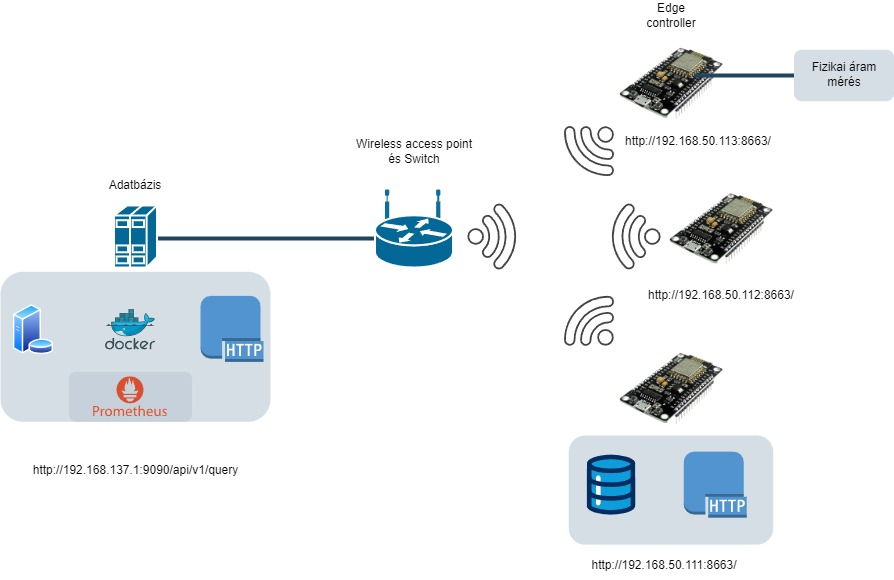
\includegraphics[width=1\textwidth]{figures/szakdoga.jpg}
    \caption{Rendszerarchitektúra}
    \label{fig:Rendszerarchitektúra}
\end{figure}

\section{Eszközök}

\subsection{Végpontok}

\subsubsection{ESP8266 és AC árammérő szenzorok}

A pontos árammérés minden elektromos töltőnél kritikus a rendszer számára. 
Az ESP8266-ot (NodeMCU) nem invazív váltakozóáram-érzékelőkkel 
párosítva használjuk a megfelelő áramkörök által felvett áramerősség mérésére. Egy megfelelő
érzékelő az YHDC SCT-013 sorozatú bilincses áramtranszformátor, például az SCT-013-030 modell, 
ami 30 A AC  feszültségre van méretezve. Az SCT-013 egy osztott magú áramváltó így könnyű a 
csatlakozása, ez a tápkábelnek feszültség alatt 
álló vezetéke köré kerül, és nincs szükség közvetlen elektromos érintkezésre a vezetővel. 
Ez az érzékelő a kábelen átfolyó árammal arányos kis váltakozó feszültséget 
ad ki. Különösen az SCT-013-030 körülbelül 0-1 V AC (effektív) kimenetet produkál 0-30 A mérésekor.
\cite{simplyexplained:emonlib}

\begin{figure}[!ht]
    \centering
    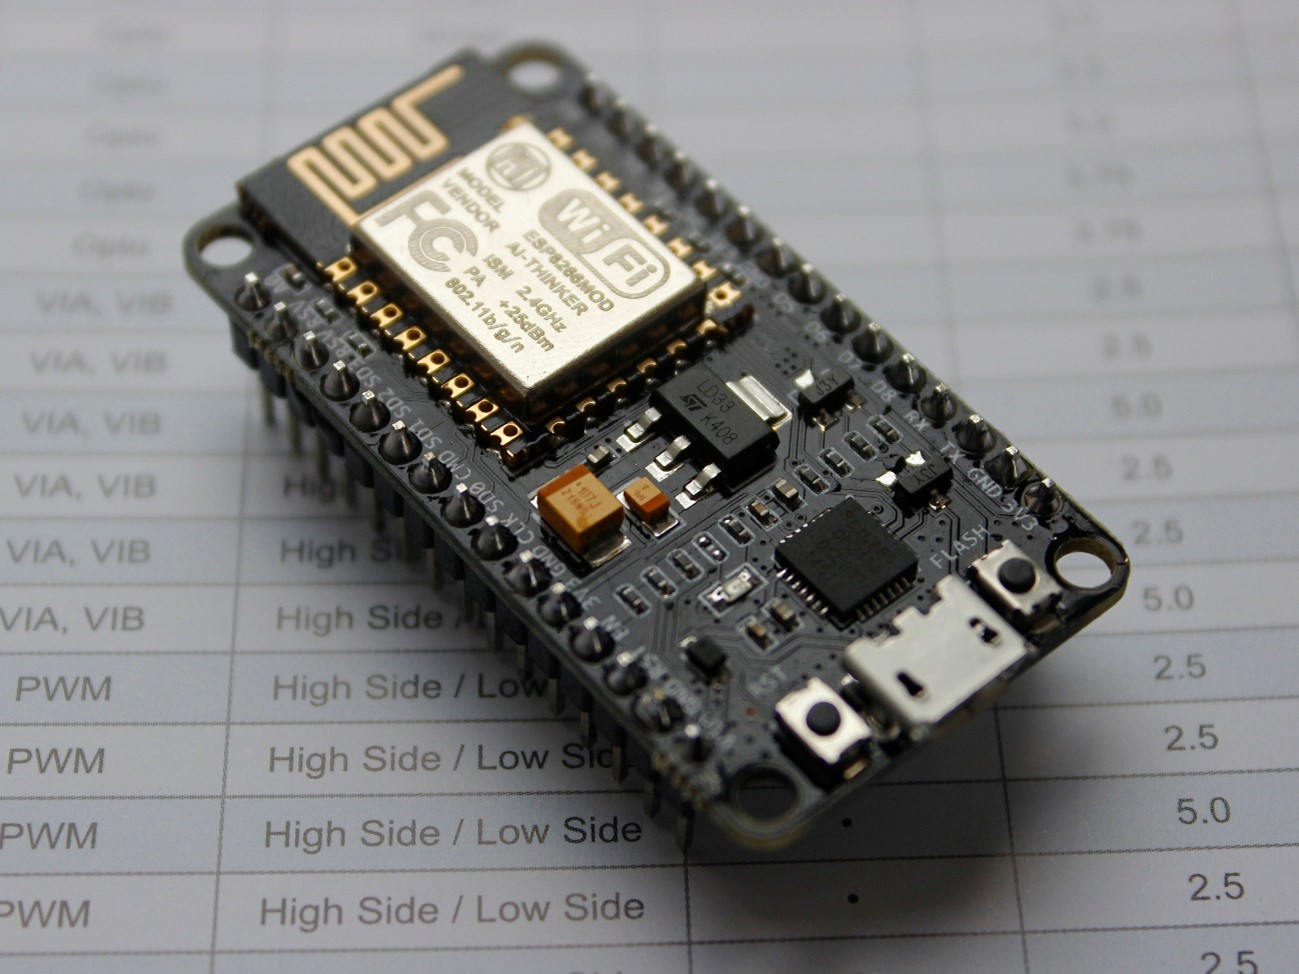
\includegraphics[width=0.8\textwidth, keepaspectratio]{figures/NodeMCU.jpg}
    \caption{NodeMCU (ESP8266) \cite{patel_nodemcu}} 
\end{figure}

Ez a feszültségtartomány kompatibilis az ESP8266 analóg-digitális átalakítójával az analóg bemenetén, 
amely a legtöbb ESP8266 kártyán 0-1 V-ot tud olvasni (a NodeMCU kártyák tartalmaznak beépített 
feszültségosztót, amely lehetővé teszi a 3,3 V-os bemenetet). Így az SCT-013-030 0-1 V-os kimenete 
közvetlenül az analóg bemenetre rakható.
Az SCT-013 érzékelők, amelyek feszültségkimenettel rendelkeznek, 
már rendelkeznek belső ellenállással, így nincs szükség további terhelésre.
\cite{openenergymonitor}

\begin{figure}[!ht]
    \centering
    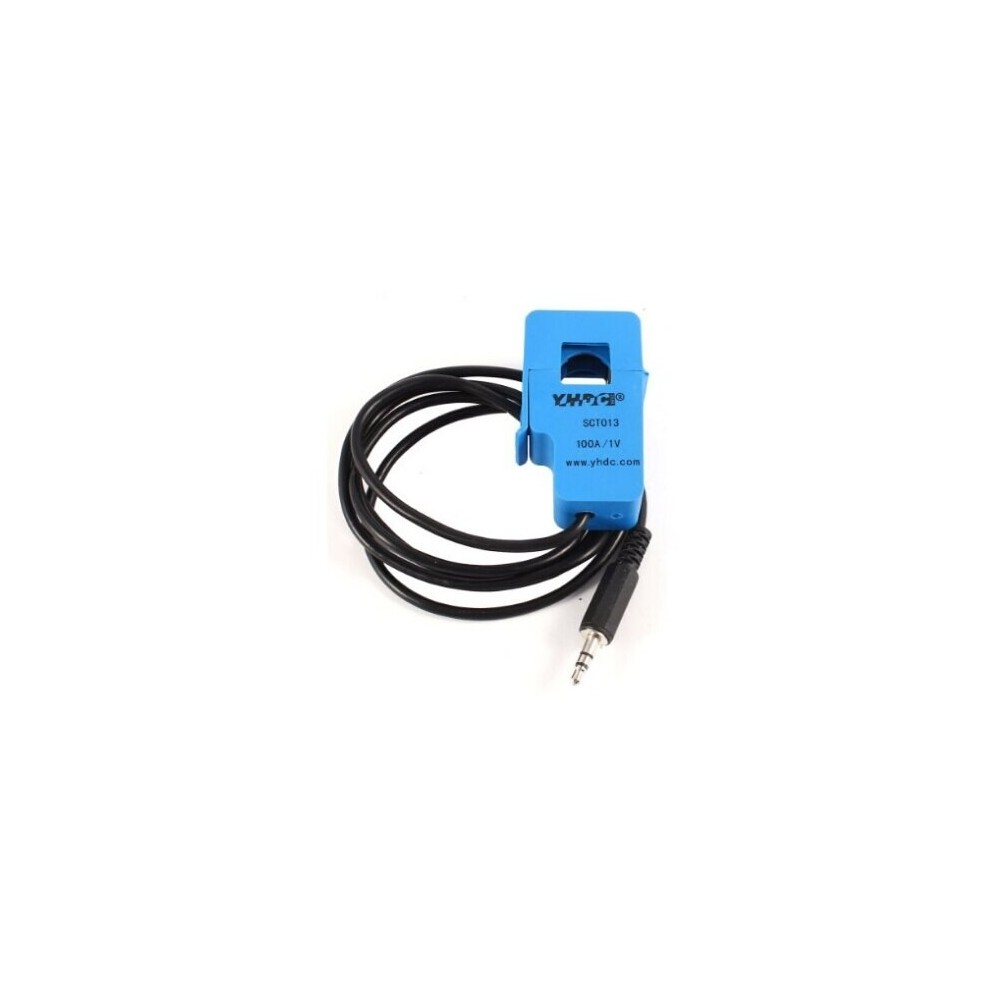
\includegraphics[width=0.8\textwidth, keepaspectratio]{figures/CT.jpg}
    \caption{SCT-013 áramváltó \cite{mikroelektronik:sct013}} 
\end{figure}

Mindkét esetben szükséges egy csatoló áramkör az érzékelőhöz: 
A CT AC kimenete 0 V ha nincsen semmi behatás, de az ESP8266 ADC nem tudja leolvasni a negatív feszültséget. 
Ezért elkell tolnunk az értékeket ehhez kell két ellenállás, amelyek feszültségosztót alkotnak 
a 3,3 V-os tápegységgel, hogy az érzékelő kimenetét a skála közepére rakjuk. 
Lényegében az érzékelő két vezetéke csatlakozik: az egyik az ADC bemenethez, 
a másik pedig a középponthoz körülbelül 1,65 V a 3,3 V-os táp miatt.
\cite{openenergymonitor}

Mindegyik ESP8266 tápellátást kap lehetőleg 5 V-os USB-adapterrel az EV-töltő kiegészítő tápellátásával 
és az analóg bemeneten keresztül olvassa le a CT-érzékelőjét.
A mikrokontroller a megírt kódot futtatja, csatlakozik a Wi-Fi-hez, és folyamatosan méri az áramerősséget. 
Ezt úgy küldi a szervernek, hogy már könnyű legyen prometheusnak tovább küldeni.

\subsubsection{Mért eszközök}

Különböző eszközök mérését hajtok végre egy hálózatban, amiknél, más paraméterek mérésére van szükségünk.

Ilyen eszközök a megszakítók, itt érzékelnünk kell:
\begin{itemize}
    \item \textbf{Megszakítók:}
    \begin{itemize}
        \item Pillanatnyi áramerősség
        \item Állapotjelzés
        \item Hibajel
        \item Túlterhelés figyelmeztetések
    \end{itemize}
    \item \textbf{Autótöltők:}
    \begin{itemize}
        \item Pillanatnyi áram
        \item Állapot (csatlakoztatva, tölt, hiba, stb...)
    \end{itemize}
    \item \textbf{Szekrények:}
    \begin{itemize}
        \item Hőmérés
        \item Gázelemzés (füst érzékelés)
    \end{itemize}
\end{itemize}

A mérések egy mikrokontrollerbe vannak beprogramozva, sok esetben, 
hogy a megfelelő és helyileg feldolgozható jelet kapjunk valamilyen hardverre van szükség, ez átalakítja az eredeti jelet. 
Ilyen például az áram méréséhez használt áramváltó és sönt ellenállás, jellemzően a nagyobb áramokat 5 A-re transzformáljuk 
egy áramváltóval.

Esetünkben maga az ESP8266 chip az analóg bemenetén 0 és 1 volt közötti jelszintet vár, 
viszont a nodeMCU környezet már végez az áramkörön feszültség áttalakítást így a bemeneti skála változik 0 és 3,3 voltra.

Ha áramméréseket áramváltóval akarjuk megvalósítani akkor az áramváltó 5 A-es maximum kimenetét kell 
a kontroller 3,3 v-os maximum bemenetére alakítani. Ezt egy sönt ellenállással tudjuk megvalósítani.


\begin{equation}
    R = \frac{U}{I} = \frac{3.3 \, \text{V}}{5 \, \text{A}} = 660 \, \text{m}\Omega
\end{equation}
\begin{center}
    \textbf{1. egyenlet:} Áramméréshez használt sönt ellenállás értéke
\end{center}
    
\begin{equation}
    P = U \times I = 3.3 \, \text{V} \times 5 \, \text{A} = 16.5 \, \text{W}
\end{equation}
\begin{center}
    \textbf{2. egyenlet:} A sönt ellenállás
\end{center}

A számítások után látszik, hogy olyan ellenállásra van szükség, ami $R = 660 m\Omega$ ellenállással rendelkezik és legalább 16,5 W 
teljesítményt el tud diszipálni folyamatos terhelés melett is.


\section{Kommunikáció}

\subsection{ESP8266 és Szerver között (Wi-Fi és REST API)}

A kommunikációhoz az ESP8266 végpontok Wi-Fi-t használnak a mérések továbbítására a vezérlő Flask szerverre. 
Indításkor minden ESP8266 csatlakozik a konfigurált 
Wi-Fi hozzáférési ponthoz. 
\begin{lstlisting}
    (pl. WiFi.begin(ssid, jelszó))
\end{lstlisting}
Itt az ESP8266 beépített WiFi könyvtárat használtam.
\cite{techtutorialsx:esp8266flask}
A csatlakozást követően a csomópont képes HTTP vagy esetünkben HTTPS kéréseket küldeni a szerver IP-címére. 
Egy egyszerű RESTful API-t implementáltam a Flask szerveren az adatok fogadásához. 
Minden fizikai végpont Prometheus adatbázis jellegű kommunikációhoz is használt végponton hirdeti a mért adatait.
\begin{lstlisting}
    app.run(host="0.0.0.0", port=6000, ssl_context=('cert.pem', 'key.pem'))
\end{lstlisting}

\begin{lstlisting}
    http://<szerver_ip>:6000/metrics
\end{lstlisting} 
A JSON adatstruktúra a következő:

\begin{lstlisting}
    def metrics():
    return jsonify({
        "simulator_id": simulator_id,
        "current": current_value,
        "state": "plugged in" if charger_on else "plugged out",
        "max_current": max_current
    })
\end{lstlisting}

A Wi-Fi kommunikáció itt nem követeli meg, hogy az ESP8266 ismerje a szerver címét, mert csak GET parancsokat
használtam. Itt a kiszolgáló fix IP-címmel rendelkezhet a LAN-ban. Elég viszont, ha a szerver ismeri a végpontok IP címeit,
amit viszont könnyű megadni és frissíteni.
Kezdetben titkosítatlan HTTP-t használtam, viszont ezt később frissítettem a valódi telepítési környezethez hasonló 
HTTPS-el. Szerencsére az ESP8266 képes kezelni a TLS-t.

\subsection{Modbus}

A vezérlő oldalon a szerver a Modbus protokollt használja az EV-töltőkkel való kommunikációhoz. 
A Modbus egy széles körben elterjedt protokoll az ipari rendszerekben elektronikus eszközök csatlakoztatására. 
Eredtileg PLC-k közötti Kommunikáció kialakítására használták.
A mi beállításunkban a szerver Modbus masterként van konfigurálva, 
és minden EV töltő Modbus slave eszköz (Modbus/TCP). A Modbuson keresztül a szerver képes regisztereket olvasni a 
töltőkről, és regisztereket írni. Ezzel áttudtam írni a töltőben a maximális áramértéket amit engedélyezett. 
\cite{mcuoneclipse:evcharger}

\begin{figure}[!ht]
    \centering
    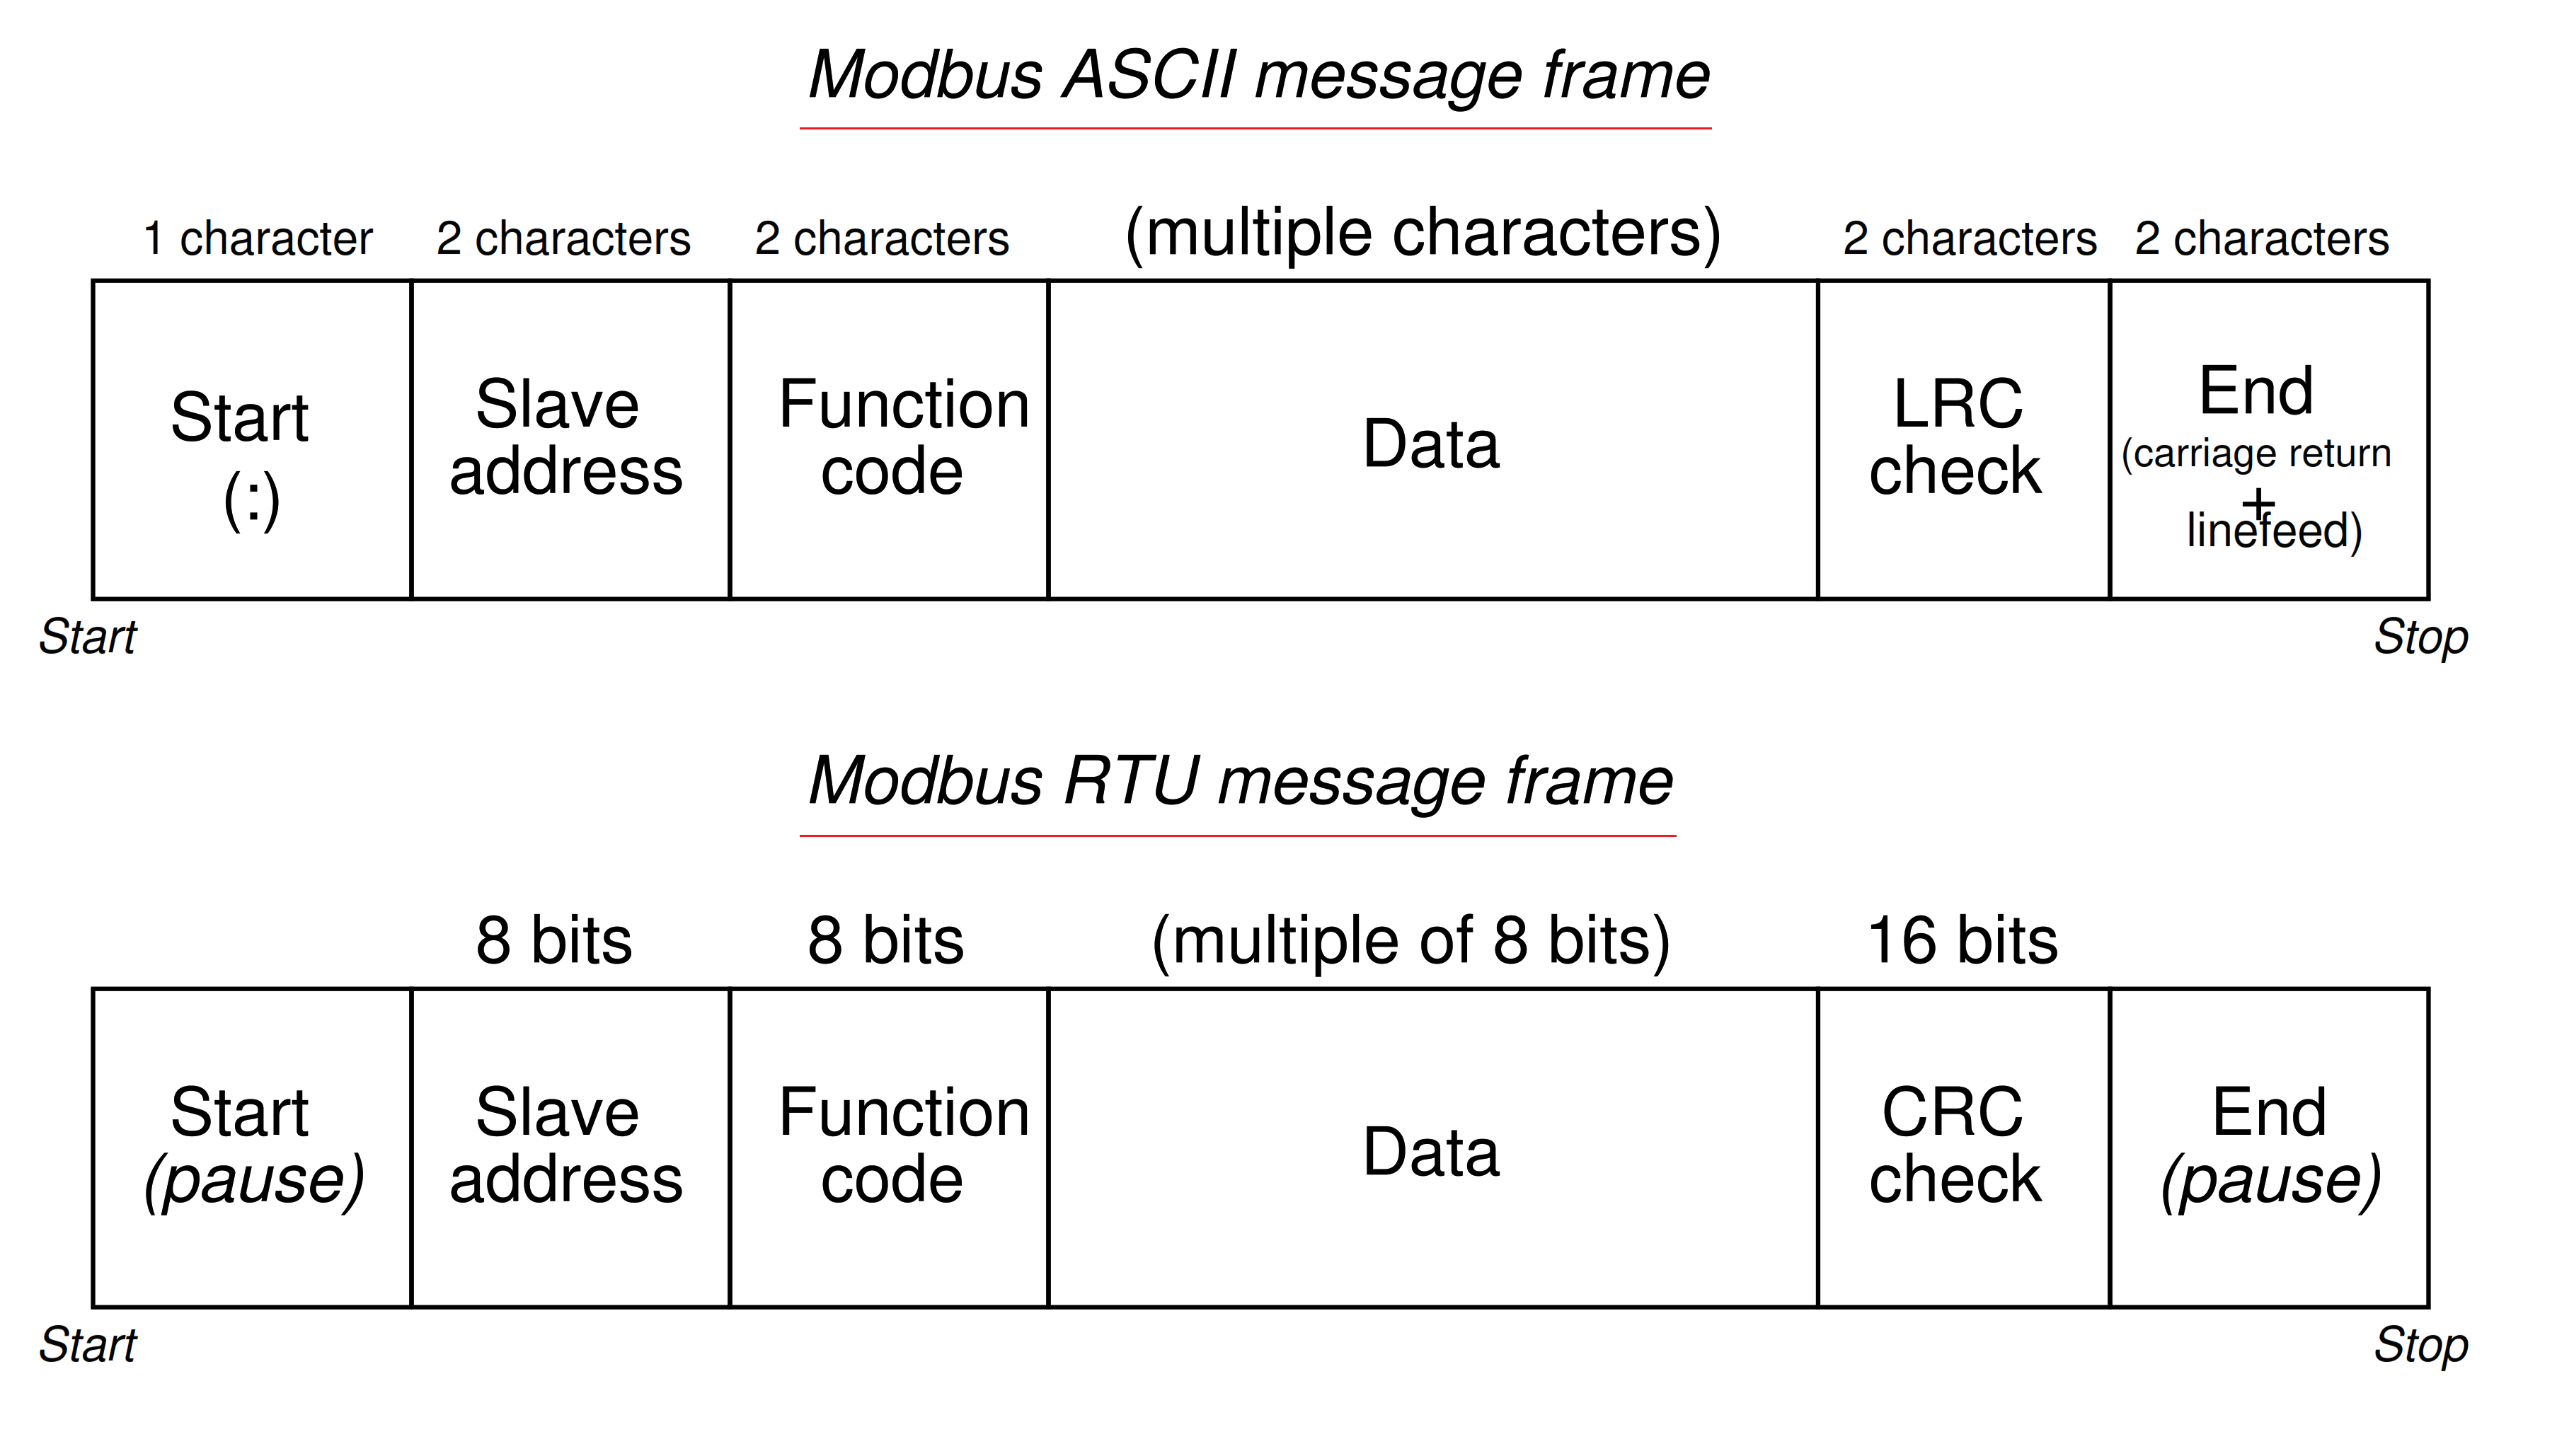
\includegraphics[width=0.8\textwidth, keepaspectratio]{figures/Modbus_Frame.png}
    \caption{Modbus adatstruktúra \cite{instrumentationtools:modbus}} 
\end{figure}

A képen Modbus RTU soros kommunikáció összeállítása látszik. Ebben a rendszerben Modbus TCP rendszert használunk.
Ez igazából csak annyit csinál, hogy TCP keretekbe foglalja a már előbb felsorolt kommunikációt.

\section{Standardizált rendszer}

\subsection{Áttekintés}

Direkt úgy állítottam össze a rendszert, hogy az moduláris, konténeres keretrendszert tudjon képezni. 
Ez így lehetővé teszi az épületek energiagazdálkodásához szükséges komponensek gyors integrációját, 
leginkább az EV-töltőkre és a megszakítópanelekre fókuszálva. Az adat tárolást (Prometheus), 
vezérlő API-kat és vizualizációt (Grafana) szabványosítja ebben az esetben, hogy egyszerűsítse a 
demo környezeteket és a termelési környezetben bevezetéseket is.

\subsection{Tervezési célok és követelmények}

\begin{itemize}
    \item Plug-and-Play alkatrészek: A felhasználók új érzékelőket vagy vezérlőket önálló szolgáltatásként telepíthet, 
    amíg az kompatibilis a keretrendszer eszközeivel.
    \item Szabványosított mérési API: Itt egyszerűen minden komponens Prometheus-formátumú metrikákat exportál HTTPS-n 
    keresztül.
    \item Vezérlő: A Python-alapú ControlServer REST protokollon keresztül irányítja az eszközöket.
    \item Konténerizált környezet: Minden mikroszolgáltatás konténerekben fut; az orchestrálást, 
    pedig Kubernetes segítségével oldottam meg.
    \item Skálázhatóság és bővíthetőség: Könnyedén skálázható ez a környezet , hozzá lehet adni új erőforrástípusokat, 
    és integrálni új eszközöket, mint ütemezés vagy akár valamilyen ML elemzés.
\end{itemize}

\begin{figure}[!ht]
    \centering
    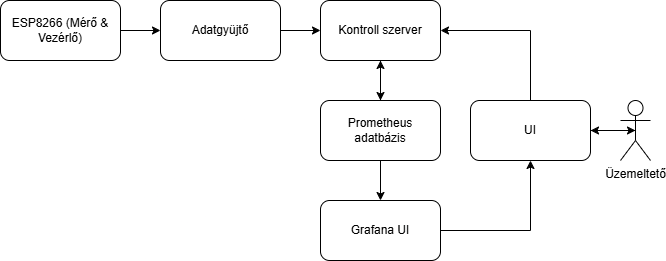
\includegraphics[width=0.8\textwidth, keepaspectratio]{figures/framework.png}
    \caption{Keretrendszer architektúra}
\end{figure}

Mivel kubernetesben telepíthető a keretrendszer minden komponense konténerként fut 
és a cluster szolgáltatásai gondoskodnak arról, hogy a Python ControlServer, az ESP8266-hoz kapcsolódó adapterek, 
valamint a Prometheus és Grafana mindig elérhetők és skálázhatók legyenek.

A Python ControlServer egy Deployment formájában jön létre, ezt egy Service köti össze a belső hálózaton belül. 
A Deployment manifest-jében TLS tanúsítványokat tartalmazó Secret hivatkozik a HTTPS tanúsítványokra, 
így minden REST hívás titkosított csatornán zajlik. A control serveren belül a Flask alapú REST API két fő végpontot kínál: 
az egyik a /metrics, ami Prometheus kompatibilis formátumban szolgáltatja az aktuális fogyasztási metrikákat, 
a másik pedig a vezérlőhívások fogadására van fenntartva ahol lehet új áramkorlátokat beállítani az EV töltők számára.

Az ESP8266 szenzorok microservice-ként jelennek meg a rendszerben: mindegyik egy Deployment, 
ami tartalmazza a hardverrel kommunikáló sorospor adaptert. 
Ezek a podok HTTPS-en jelentkeznek be a ControlServernél, és folyamatosan kiszolgálják a /metrics végpontjukat. 
A Prometheus-ban lekonfiguráljuk, hogy a Prometheus scrapper felvegye őket a targetek közé. 
A felhasználó, ha új eszközt telepít és megadja a prometheus.io/scrape: "true" és prometheus.io/path: "/metrics" értékeket. 
Így plug and play módon csatlakozható tetszőleges új érzékelők vagy vezérlők.

A Prometheus egy StatefulSet formájában fut és PersistentVolumeClaim segítségével tárolja el az adatbázist, 
így újraindítás esetén se vesznek el az adatok. A scrape konfiguráció paraméterezését ConfigMapben lehet megtenni. 
A Grafana Deployment mellé szintén egy PVC került a dashboard-ok mentéséhez 
és ConfigMapeken keresztül lehet dashboard-okat definiálni. Az útválasztó SSL-terminációja 
után a felhasználó hozzá fér az irányítópulthoz.

A skálázhatóságot HorizontalPodAutoscaler biztosítja: ha egy pod CPU- vagy memóriahasználata átlépi a beállított küszöböt, 
Kubernetes automatikusan podokat indít. Ez a felépítés lehetővé teszi, 
hogy a cluster pillanatnyi terhelésének megfelelően bővítsük a kapacitást, akár kibőtve külső linux VM-re.